%%%%%%%%%%%%%%%%%%%%%%% file typeinst.tex %%%%%%%%%%%%%%%%%%%%%%%%%
%
% This is the LaTeX source for the instructions to authors using
% the LaTeX document class 'llncs.cls' for contributions to
% the Lecture Notes in Computer Sciences series.
% http://www.springer.com/lncs       Springer Heidelberg 2006/05/04
%
% It may be used as a template for your own input - copy it
% to a new file with a new name and use it as the basis
% for your article.
%
% NB: the document class 'llncs' has its own and detailed documentation, see
% ftp://ftp.springer.de/data/pubftp/pub/tex/latex/llncs/latex2e/llncsdoc.pdf
%
%%%%%%%%%%%%%%%%%%%%%%%%%%%%%%%%%%%%%%%%%%%%%%%%%%%%%%%%%%%%%%%%%%%
\documentclass[11pt,oribibl,runningheads]{llncs}
\usepackage[a4paper,hmargin=1in,vmargin=1.25in]{geometry}

%\documentclass[]{llncs}

\usepackage{amssymb}
\usepackage{amsmath}
\setcounter{tocdepth}{3}
\usepackage{graphicx}
\usepackage{subfig}
\usepackage{alg}


\usepackage{url}
\urldef{\mailsa}\path|orlandi@daimi.au.dk |
\urldef{\mailsb}\path|{piva, caini}@lci.det.unifi.it |
\urldef{\mailsc}\path|barni@dii.unisi.it|
\newcommand{\keywords}[1]{\par\addvspace\baselineskip
\noindent\keywordname\enspace\ignorespaces#1}

\begin{document}

\mainmatter  % start of an individual contribution

% first the title is needed
\title{Enhancing Privacy in Remote Data Classification}

% a short form should be given in case it is too long for the running head
%\titlerunning{Lecture Notes in Computer Science: Authors' Instructions}

% the name(s) of the author(s) follow(s) next
%
% NB: Chinese authors should write their first names(s) in front of
% their surnames. This ensures that the names appear correctly in
% the running heads and the author index.
%
\author{Claudio Orlandi\inst{1}\thanks{Work done while working at University of Florence.}\and Alessandro Piva\inst{2} \and Michele Caini\inst{2} \and Mauro
Barni\inst{3}}
%
%\authorrunning{Lecture Notes in Computer Science: Authors' Instructions}
% (feature abused for this document to repeat the title also on left hand pages)

% the affiliations are given next
\institute{Department of Computer Science, University of Aarhus; \\
\mailsa\\  \and Department of Electronics and Telecommunications,
University of Florence; \\ \mailsb\\
 \and
Department of Information Engineering, University of Siena;\\
\mailsc }

%
% NB: a more complex sample for affiliations and the mapping to the
% corresponding authors can be found in the file "llncs.dem"
% (search for the string "\mainmatter" where a contribution starts).
% "llncs.dem" accompanies the document class "llncs.cls".
%

%\toctitle{Lecture Notes in Computer Science}
%\tocauthor{Authors' Instructions}
\maketitle


\begin{abstract}

Neural networks are a fundamental tool in data
classification since they represent a universal tool enabling a
great variety of applications. A protocol whereby a user may ask
a service provider to run a neural network on an input provided in
encrypted format is proposed here, in such a way that the neural
network owner does not get any knowledge about the processed data. At the same
time, the knowledge embedded within the network itself is
protected.

With respect to
previous works in this field, the interaction between the user and
the NN owner is kept to a minimum without resorting to general secure multi-party
computation protocols.

\keywords{Privacy-Preserving Computation, Neural Networks,
Homomorphic Encryption, Signal Processing in Encrypted Domain,
CryptoComputing}
\end{abstract}


\section{Introduction}

Recent advances in signal and information processing together with
the possibility of exchanging and transmitting data through
flexible and ubiquitous transmission media such as internet and
wireless networks, have opened the way towards a new kind of
services whereby a provider sells its ability to process and
interpret data remotely, e.g. through an internet web service.
Examples in this sense include access to remote databases,
processing of personal data, processing of multimedia documents,
interpretation of medical data for remote diagnosis. In this last
scenario, a patient may need a diagnosis from a remote medical
institute that has the knowledge needed to perform the diagnosis.
Health-related data are of course sensitive, and the patient may
do not want to let the institute to know the data he owns; on the
other hand, the medical institute is interested in protecting his
expertise.

In 2000 two different papers proposed the notion of privacy
preserving data mining, meaning the possibility to perform data
analysis on a distributed database, under some privacy
constraints. Lindell and Pinkas \cite{PPDM-LindellPinkas}
presented a way to securely and efficiently compute a decision
tree using cryptographic protocols; at the same time, Agrawal and
Srikant \cite{PPDM-Agrawal} presented another solution to the same
problem using data randomization.

After the publication of these papers, security constraints were added to several techniques from
machine learninn, including: decision
trees \cite{PPDM-LindellPinkas}, neural networks
\cite{chang2005ope}, support vector machines \cite{lipmaa2006svm},
naive bayes classifiers \cite{kantarcioglu03privacy}, belief
networks \cite{yang2005bayesian,wright2004bayesian}, clustering
\cite{jha2005ppc}. In all these works, we can identify two major
scenarios: in the first one Alice and Bob share a dataset and want
to extract knowledge from it without revealing their own data
(privacy preserving data mining). In the other scenario, which is
the one considered in this paper, Alice owns her private data $x$,
while Bob owns an evaluation function $C$ (in most cases $C$ is a
classifier). Alice is interested in having her data processed by
Bob, but she does not want that Bob learns either her input or the
output of the computation. At the same time Bob does not want to
reveal the exact form of $C$, representing his knowledge, since,
for instance, he sells a classification service through the web
(as in the remote medical diagnosis example).

A fundamental brick in data classification task is represented by
neural networks (NNs), becayse of their approximation and
generalization capabilities. For this reason, it can be of interest to
design a protocol whereby a user may ask a service provider to
run a neural network on an input provided in encrypted format.
Previous works on privacy preserving NN computing are limited to
the systems presented in \cite{ppnn,chang2005ope}. However, such
studies resort extensively to highly inefficient general secure
multi-party computation (SMC) \cite{Yao86} for
the computation of the non-linear activation functions implemented
in the neurons.

This is not the case with our new protocol which does not resort
to general SMC for the evaluation of the activation functions. In
a nutshell, the protocol has been designed to ensure that the data
provided by the user (say Alice), representing the input of the
neural network are completely protected and, at the same time, to
not disclose Bob's classifier (the NN). The proposed protocol relies on homomorphic encryption
that allows to perform directly in the encrypted domain all the
linear computations. For the non linear functions that can not be
handled by means of homomorphic encryption, a limited amount of
interaction between the NN owner and the user is introduced to
delegate the user (say Alice) to perform some of the computation.

Comparing our work with previous ones, another advantage can be
highlighted: the proposed protocol can handle every kind of
feedforward NN (not only simple layered networks), without
disclosing neither the number of neurons nor the way they are
connected.

The rest of this paper is organized as follows. In Section
\ref{sec.NN}, a brief overview on Neural Networks that can be used
with our protocol is given. In Section
\ref{sec:RDC} our scenario will be described, focusing on the
privacy constraints and reviewing the properties to be achieved
by our protocol. The way the protocol works is described in
Section \ref{sec:protocol}. Section \ref{sec:exp} is devoted to
the experimental results obtained developing a distributed
application that runs the protocol. Some concluding remarks are
given in Section \ref{sec:conclusion}, while in Appendix how to deal with non integer computation will be
discussed.

\section{Neural Networks}
\label{sec.NN} Neural networks have a great
ability to model any given function \cite{lapedes1988nnw,70408}. Moreover neural networks
are provided with good learning algorithms, are robust
against noise and generalize well on unseen examples.

In this section we will introduce several types of network that
can be used with our protocol. The notation is consistent with the
one in \cite{bishop1995nnp}, where a detailed treatment of neural
networks functioning and applications is given.

\subsection{Perceptron}
The simplest neural network is the {\em perceptron} (Figure
\ref{networks} (a)). It can discriminate between two different
classes of instance, and its classification function consists of a
linear combination of the input variables, the coefficients of which
are the parameters of the model. The discriminant is of the form $ a(\vec{x})=\vec{w}^T\vec{x} + w_0 $
where $\vec{x}$ is the input vector, $\vec{w}$ is the vector of
weights and $w_0$ is a threshold\footnote{From now on we can forget about $w_0$ simply appending it at the end of the vector and obtaining $a(\vec{x})=[\vec{w} \ w_0]^T[\vec{x} \ 1]$}. The instance $\vec{x}$ is assigned
to class $c_1$ if $a(\vec{x}) \geq 0$ and to class $c_2$ if
$a(\vec{x})<0$.  This method can easily be extended to the multiclass case using
one discriminant function $a_k(x)$ for each class $C_k$ such that
$a_k(\vec{x})=\vec{w}^T_k\vec{x}$.

\subsection{Feed-Forward Networks}
To allow for more general classification we consider a network of interconnetted neurons.

\paragraph{Layered Networks.}
Networks consisting of successive layers of adaptive weights are
called {\em layered networks}: in such a network every unit in one
layer is connected to every unit in the next layer, but no other
connections are permitted, as shown in Figure \ref{networks} (b)
The units that are not treated as output units are called {\em
hidden} units.

The output of the $j$-th hidden unit in the $i$-th layer is
obtained by first forming a weighted linear combination of its $l$
input values to give
$$
a^{(i)}_j = \sum_{k=1}^l w^{(i)}_{jk}x_k
$$
Here $w_{jk}^{(i)}$ denotes the weight associated to an edge going
from the $k$-th neuron of the previous layer to the neuron $j$ of
$i$-th layer. The activation of the hidden unit is then obtained
by transforming the linear sum using an activation function
$g(\cdot)$ to obtain $z^{(i)}_j=g\left(a^{(i)}_j\right)$.

This procedure is iterated until the output layer is reached,
obtaining the final output $y_k = g(a_k)$.

We will refer to a $L$-layer network as a network having $L$
layers of adaptive weights, regardless of the input units.

\paragraph{General topologies.}
Since there is a direct correspondence between a network diagram
and its mathematical function, we can develop more general network
mappings by considering more complex network diagrams. To be able to run the computation,
however, we shall restrict our attention to the case of {\em feed-forward}
networks, in which there are no feed-back loops, as shown in Figure
\ref{networks} (c).
%
\begin{figure}[t]
\centering
%\psfig{figure=img/perceptron.eps,width=8.5cm}
\subfloat[Perceptron]{
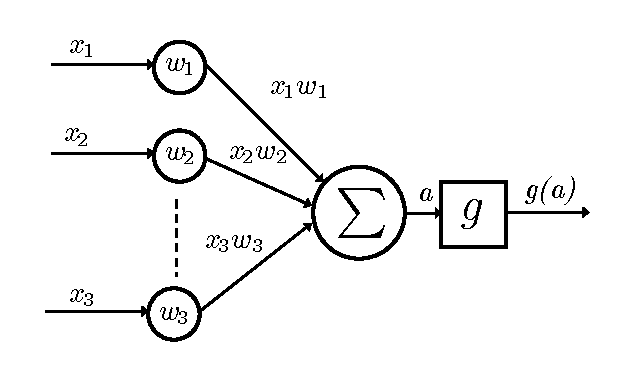
\includegraphics[width=0.5\textwidth]{img/perceptronbb.eps}}
\qquad \subfloat[Multilayer network]{
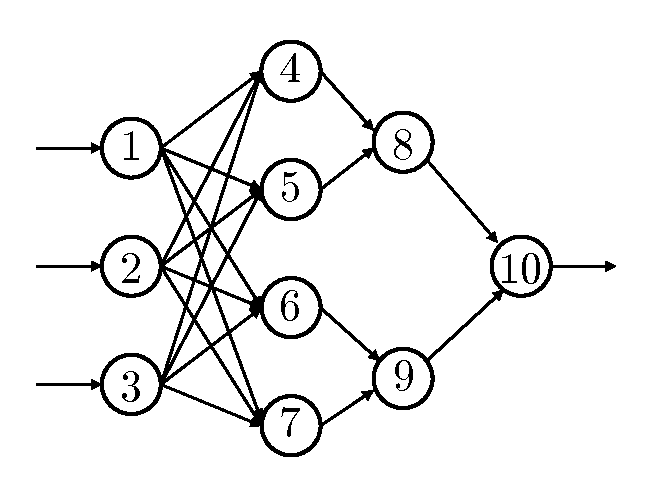
\includegraphics[width=0.35\textwidth]{img/networkbb.eps}}
\qquad \subfloat[General feedforward network]{
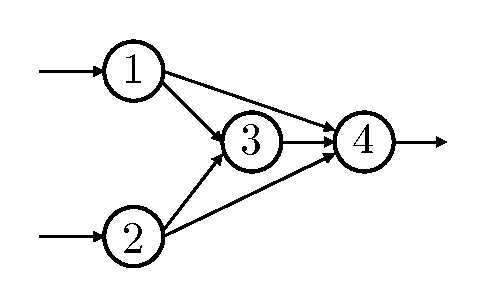
\includegraphics[width=0.35\textwidth]{img/nonlayeredbb.eps}}
\caption{Three kinds of different networks that can be used with
the proposed protocol. Figure (a) shows a single layer network,
known as {\em perceptron}; Figure (b) shows a {\em multi-layer
feedforward network }, while Figure (c) shows a {\em general
feedforward network.} Note that in feed-forward networks it is
possible to number neurons such that every neuron gets inputs only
from neurons with smaller index. }\label{networks}
\end{figure}
%
\paragraph{Activation Function.}
The activation function of the hidden neurons are usually
sigmoidal functions, i.e. $g(a)= \frac{1}{1+e^{-a}}$.

The differentiability of this kind of functions leads to a
powerful and computationally efficient learning method, called
{\em error backpropagation} {\cite{rumelhart1986lir}}.

We allow output neurons to have both sigmoid activation functions or
linear activation functions. The latter is sometimes desirable
because the use of sigmoid units at the outputs would limit the
range of possible outputs to the range attainable by the sigmoid.

\section{Remote Data Classification}
\label{sec:RDC}The scenario we are going to consider is the
following: Alice owns a vector of data, while Bob owns a
classifier. Alice is interested to classify her data by exploiting
Bob knowledge.

There are two trivial solutions for this problem: Alice sends her
data and Bob performs the classification, or Bob sends his
classifier and Alice performs the classification. Both these
solutions have a clear drawback. Alice don't want to
disclose Bob her data or the output of the classification (in
the case of the previous medical example, Alice don't want to
reveal Bob if she is actually healthy or not). On the other
hand, Bob might not be happy to disclose the classifier, since he
probably invested time and money training his
network.

Again we can find a trivial solution, that is to find a trusted
third party (TTP) that takes inputs from Alice and Bob, and gives
 back to Alice the output of the computation. Of course this
scenario is not the ordinary one. If Alice and Bob distrust each
other, it could be hard to find a common TTP.

Our goal is to design a protocol for remote data classification
that respects the above privacy constraints without resorting to a
TTP, and where cryptography and some randomization will play the
role of the TTP. As many other protocols in literature, we will make
the assumption that both Alice and Bob are semi-honest. This means
that they will follow the protocol properly, but they can later
analyze the protocol transcript trying to discover information
about other party inputs.
We will also assume that Alice and Bob
can communicate over a secure (private and authenticated) channel, that can be implemented in practice as a
standard SSL connection.

To grant protection against malicious adversary (i.e. adversary
that can behave differently from what they are supposed to do),
there are standard constructions to produce a protocol secure in
the malicious scenario from a semi-honest one
\cite{Gold87}. Moreover in our protocol, there is no
evidence that a cheating player can discover significant
information about other party inputs, and therefore we can assume that semi-honest behaviour is forced 
by external factors i.e. Bob being a service provider
doesn't want to lose his reputation, and Alice is interested in having her data correctly classified.


\subsection{Protocol Requirements}

\paragraph{Correctness.}
 It means that Alice wants to have a
    correct classification of her data. As Bob gets no output, only Alice has
    interest in this property. We are not concerned here
    with the accuracy of Bob's NN, nor we could be.
    What we mean here is that Bob could maliciously give an incorrect answer to Alice, i.e.
in the medical example, a corrupted Bob is instructed to reply ``ill'' to a given list of
    people. We could avoid this kind of cheating by running our protocol over an anonymized network as is \cite{tor-design}.
 In general as our protocol is only secure against semi-honest
    adversaries, we can't ensure correctness: to do so,
    we have to transform our protocol into a protocol secure
    against malicious adversary using standard compiler techniques \cite{Gold87}.


\paragraph{Alice's Privacy.}
Alice's data are completely protected. In fact, Alice gives her input in an
    encrypted format and receives the output in an encrypted
    format. So Alice's privacy relies on the security of the
    underlying cryptosystem that is, in our case, semantic security.

\paragraph{Bob's Privacy.}
While it's clear what we mean with Alice's privacy, it's not the
same with Bob's privacy. We need again to refer to the TTP ideal
scenario: as long as Alice gets her data classified, she's learning
something about Bob classifier. She learns in fact how Bob
classifies a vector data. Suppose that she runs the protocol an
arbitrarily number of times: she can submit every (or
a very large database of) instances to be classified by Bob. She
can later easily build a table with the classification of every
vector, building in that way a classifier that works the same of
Bob's one for classified vector, and she will be able to
classify also new vectors, maybe building a new neural network
with this data as the training set.

This result does not depend on the protocol security (we are
talking about the TTP ideal scenario) but simply on the fact that
from the input and the output of a computation it is always
possible to learn something about the computed function (and this
is exactly the goal of machine learning).

A natural question is therefore: is it possible to model this kind of attack, where a user interact many times with the classifier to understand his structure? How many interactions do the attacker needs? This question is partially answered in watermarking literature under the name ``sensititvity attack''.
For a linear classifier (perceptron) the number of
iterations to completely disclose it is very low
\cite{Cox97,Kalk98}. For a more complex function, like a
multi-layer network, it's harder to say, but there are still
solutions allowing to extract a local boundary even without
knowing anything about the nature of the classifier
\cite{comesana2006bns}.

Here is what our protocol protects about Bob's NN:
\begin{description}
    \item[Structure of the Network:] Bob network is composed of a
    certain number of neurons, connected in some feed-forward way.
    The protocol is designed to completely protect the way the neuron are
    connected, and to partially protect the number of neurons
    actually present in the network, so that Alice will get an upper bound $B$ for
    the number of neurons. Bob can adjust this bound $B$ in a way to
    achieve a good level of privacy and at the same time an
    efficient protocol.
    \item[Hidden Neurons Output:] we also have to protect the
    outputs of the hidden neurons, as this is an unneeded leakage of information.

    Given a hidden neuron with sigmoid activation
    function, it is possible to split its output in two parts,
    one that we can perfectly protect, while the other will be
    partially disclosed.
    \begin{itemize}
        \item {\em State of the Neuron:} this is the most important part of the output. Depending on the sign of
        the weighted sum of the inputs, every neuron can be {\em
        on}
        (i.e. output $>0.5$) or {\em off} (i.e. output $<0.5$). We
        will perfectly protect this information, flipping it with
        probability one half, achieving a one-time pad kind of security.
        \item {\em Associated Magnitude:} the activation of every
        neuron has also a magnitude, that gives information about
        ``how much'' the neuron is {\em on} or {\em off}. We will
hide those values in a large set of random values, in such a way that Alice will not learn
which values are actually part of the computation and which ones are just random junk. Of course the bigger
the set is, the more privacy it comes, and more computational resources are needed.
	\item {\em Neuron's Position:} the last trick to achieve security is to completely randomize the position of the hidden neurons in such a way that Alice will not discover which outputs correspond to which neurons. Therefore Alice may learn a bit of information at every execution (meaning something about the magnitudes of them), but she'll not be able to correlate those information in order to gain advantage from repeated execution of the protocol.
    \end{itemize}

\end{description}

\paragraph{Round Complexity.} We would like to run the computation with no interaction (except the minimum needed to input the vector and get the output). Unluckily, there are only few kinds of
algorithms that can be computed in such a way, that is $NC^1$
circuits \cite{sander1999nic}, and $NLOGSPACE$ problem
\cite{beaver2000mls}. Our protocol has a constant round
complexity, that is the
number of layers of the network.

\section{Privacy-Preserving Protocol for Remote Data Classification}
\label{sec:protocol}
We will continue to use the notation introduced before, together with some
new symbols to refer to the encrypted versions of the data. The
input of the neuron is $\vec{x}$ and its encrypted version is
$\vec{c}$, while the encrypted version of the activation $a$ of
every neuron will be referred as $d$.

\subsection{Building blocks}
\label{sec.bb}
\paragraph{Homomorphic Encryption.}
The chosen cryptosystem to instantiate our protocol is the
Damg{\aa}rd-Jurik modification \cite{rd-generalisation} of the
Paillier encryption scheme \cite{Pailler99}.

This cryptosystem is based on the hardness to decide the $n$-th
residuosity of elements modulo $n^{s+1}$, where $n$ is an RSA
modulo. At the end, the encryption and the decryption procedures
are the following:

\textbf{Set-up:} select $p,q$ big primes. Let $n=pq$ be the public
key, while the secret key, called $\lambda$, is the least common
divisor between $(p-1)$ and $(q-1)$.

\textbf{Encryption}: let $m \in \mathbb{Z}$ be the plaintext, and
$s$ such that $n^s > m$. Select a random value $r \in
\mathbb{Z}^*_{n^s}$; the encryption $c$ of $m$ is:
$$
c= E_{pk}(m,r) = (1+n)^m r^{n^s} \mod {n^{s+1}}
$$

\textbf{Decryption}: the decryption function $D_{sk}$ depends only
on the ciphertext, and there is no need to know the random $r$ in
the decryption phase. We refer to the original paper for the
complete description.

The main advantage of this cryptosystem is that the only parameter
to be fixed is $n$, while $s$ can be adjusted according to the
plaintext. In other words, unlike other cryptosystems, where one has
to choose the plaintext $m$ to be less than $n$, here one can choose
an $m$ of arbitrary size, and then adjust $s$ to have $n^s
> m$ and the only requirement for $n$ is that it must be unfeasible to find its factorization.

The trade-off between security and arithmetic precision is a crucial
issue in secure signal processing applications. As we will describe
in Appendix, a cryptosystem that offers the
possibility to work with an arbitrary precision allows us to neglect
that the cryptosystem works on integer modular numbers, and we can
consider this cryptosystem as an arbitrarily accurate non-integer
homomorphic encryption scheme.

For the sake of simplicity from now on we will indicate the
encryption just as $c=E(m)$, as the keys are chosen once and are
the same for all the protocol length, and the random parameters
$r$ are just to be chosen at random. If $x_1=x_2$ we will write
$E(x_1) \sim E(x_2)$. The encryption of a vector
$\vec{c}=E(\vec{x})$ will be simply the vector composed of the
encryption of every component of the plaintext vector.

As said, this cryptosystem satisfies the homomorphic property so,
given two plaintexts $m_1$ and $m_2$, the following equalities are
satisfied:
\begin{equation}
    D(E(m_1)\cdot E(m_2))=m_1+m_2
\label{eq.hom1}
\end{equation}
%
and
%
\begin{equation}
    D(E(m)^a)=am.
\label{eq.hom2}
\end{equation}

\paragraph{Privacy Preserving Scalar Product (PPSP).} A
secure protocol for the scalar product allows Bob to compute an
encrypted version of the scalar product between an encrypted
vector given by Alice $\vec{c}=E(\vec{x})$, and one vector
$\mathbf{w}$ owned by Bob. The protocol guarantees that Bob gets
nothing, while Alice gets an encrypted version of the scalar
product that she can decrypt with her private key. Such a protocol
is easily achievable exploiting the two homomorphic properties
(see Equations \ref{eq.hom1} and \ref{eq.hom2}):
%
\begin{algorithm}
%
\label{alg:PPSP}
 \alginout{$\mathbf{c}=E(\mathbf{x})$; Bob: $\mathbf{w}$}
 {Alice: $d=E(\vec{x}^T\vec{w})$}
 \algname{PSPP}{$\mathbf{c}$;$\mathbf{w}$}
%
\begin{algtab}
Bob computes $d = \prod_{i=1}^N c_i^{w_i}$ \\
Bob sends $d$ to Alice \\
\end{algtab}
\end{algorithm}
%

After receiving $d$, Alice can decrypt this value with her private
key to obtain the weighted sum $a$.

It is worth observing that though the above protocol is a secure one
in a cryptographic sense, some knowledge about Bob's secrets is
implicitly leaked through the output of the protocol itself. If, for
instance, Alice can interact $N$ times with Bob (where
$N=|\mathbf{x}|=|\mathbf{w}|$ is the size of the input vectors), she
can completely find out Bob's vector, by simply setting the input of
the $i$-th iteration as the vector with all $0$'s and a $1$ in the
$i$-th position, for $i = 1, \ldots, N$. If we use the scalar
product protocol described above to build more sophisticated
protocols, we must be aware of this leakage of information. This is
again a {\em sensitivity attack}, as introduced before. Note that
the problems stemming from sensitivity attacks are often neglected
in the privacy preserving computing literature.

\paragraph{Evaluation of the Activation Function}

If the function $g$ is known and
it's invertible, like in the case of the sigmoid function, the information given by $a$ or $y=g(a)$ is the same. So  Bob can simply give $a$ to
Alice that can compute $y$ by herself.

\subsection{Perceptron Protocol}
\label{sec.PP}

Now we have described all the tools that allow us to run a privacy
preserving remote data classification protocol for a single layer
network. The network has $I$ inputs and $1$ output. If the network
has more than one output neuron, say $O$, just run in parallel $O$
instances of the following protocol.

\begin{algorithm}
%
\label{alg:Percpetron}
 \alginout{$\mathbf{c}=E(\mathbf{x})$; Bob: $\mathbf{w}$}
 {Alice: classification of $\vec{x}$}
 \algname{Percpetron}{$\mathbf{c}$;$\mathbf{w}$}
%
\begin{algtab}
Alice and Bob run the \textsc{PPSP} protocol.\\
Alice decrypts the output $a=D(d)$ \\
Alice computes $g(a)$\\
\end{algtab}
\end{algorithm}
%

\subsection{Handling with Hidden Neurons}
We consider now the more interesting case of a feedforward network.

As already defined, a feedforward network is composed by $N$ neurons
that can be ordered in a way that neuron $j$ gets in input the
output of a finite set $I_j$ of neurons having index lower than $j$,
like the ones in Figure \ref{networks}. We use this ordering to
label every neuron. The weight of the connection from neuron $i$ to
neuron $j$ is indicated by $w_{ij}$. The input vector of neuron $j$
is $\vec{x}_j$ while the associated weights vector $\vec{w}_j$. So now we need to protect the output of hidden neurons and the network topology.

\paragraph{Hidden Neurons Output Protection.} In the perceptron
protocol, Bob gives to Alice the linear sum $a$ of the output
neurons, and then Alice computes by herself the activation
function output. The simple iteration of the perceptron protocol
for every neuron in the network will disclose the activation
value of every hidden neuron, but Alice is not supposed to get
this information. The activation of every $a$ can be viewed as
$a=sign(a)\cdot |a|$. Depending on $sign(a)$ the output of the
sigmoid function will be ``almost 1'' (i.e. $0.5 \leq y < 1$) or
``almost 0'' (i.e. $0 < y \leq 0.5$). We can perfectly protect
$sign(a)$ by exploiting the fact that the sigmoid function is
actually antisymmetric as shown in Figure \ref{sigmoid}, i.e.
$g(-a)=1-g(a)$.

Bob can randomly change the sign of $a$ just before send it to
Alice thanks to the homomorphic property, since $E(a)^{-1}=E(-a)$.
Then Alice can decrypt as usual the value received, compute the
activation function on the received input $g(-a)$ and send
$E(g(-a))$ back to Bob. Bob can recover the value he needs simply
performing the subtraction, that is
$E(g(a))=E(1-g(-a))=E(1)E(g(a))^{-1}$. In this way Alice will not
discover which (nor how many) neurons are actually activated or not. We will deal
with the protection of the value $|a|$ later.

\begin{figure}
\centering
 \includegraphics[width=0.35\textwidth]{img/sigm.eps} \\
\caption{Sigmoid functions is antisymmetric with respect to
$(0,1/2)$ as shown. That is $g(-a)=1-g(a)$.}
%
\label{sigmoid}
\end{figure}

\paragraph{Network Embedding.}
To protect the network topology, i.e. the number of neurons and
the way they are connected, we will embed the network in a
multilayer network, composed of $L$ layers of $M$ neurons each. Of
course $LM \geq N$. The added $LM - N$ neurons will be called {\em
fake neurons}. They have to look the same of the real neuron and
so they will be initialized with some incoming connection from
other neurons, with random weights. They will not influence the
computation as no real neurons will take their output as input.

A good embedding is one where every neuron only get inputs from
neurons that are in previous layers. An example of a legal embedding
of the network in Figure \ref{networks} (b) is given in Figure
\ref{embedding}.

In this way Alice will only learn an upper bound $LM$ for the
actual number of neurons $N$, while she will not learn the way
they are connected or the connection weights, as Bob can perform
the \textsc{PPSP} for every neuron by himself just picking up the
necessary inputs and make the weighted sum with his private
weights. The number $L$ also gives a bound about the longest path
between input and output neurons. Instead $M$ is not the upper bound of the incoming connection for a neuron, given that 
we can split one original layer into two or more layer in the embedded network. Every neuron in layer $l$ can take inputs from any neuron belonging to any previous layer.

The more we increase $L$, the more we protect the network topology. At the same
time $L$ will be the number of interaction round of the protocol, so
we have to find a tradeoff between round complexity and network
topology protection. 

\begin{figure}
\centering

\subfloat[Network
Embedding]{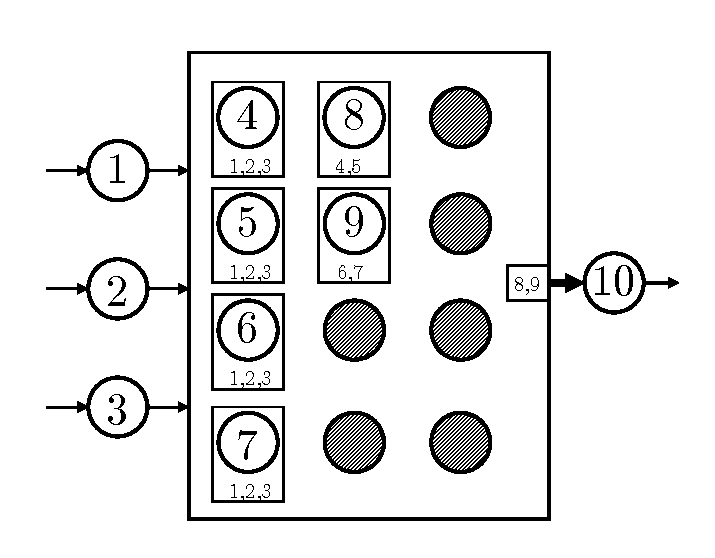
\includegraphics[width=0.45\textwidth]{img/embeddingbb.eps}}
\qquad \subfloat[Network
Scrambling]{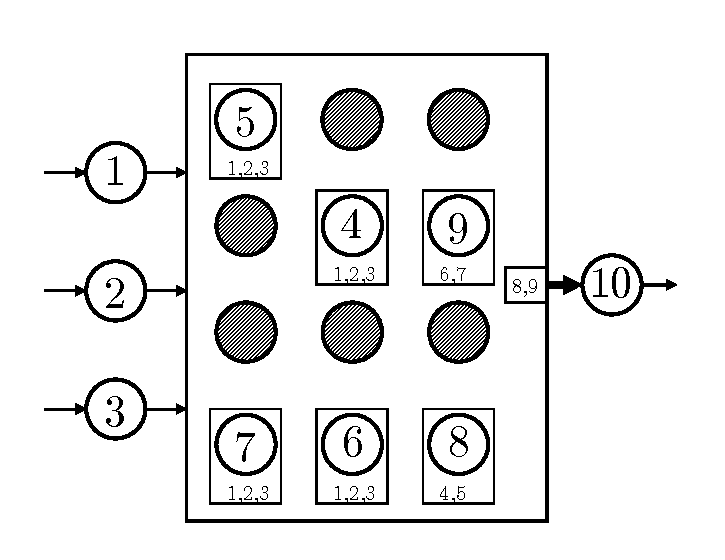
\includegraphics[width=0.45\textwidth]{img/scramblingbb.eps}
}
 \caption{Figure (a) is a natural embedding of the network in Figure \ref{networks} (b) into
a $3\times 4$ network. The big box refers to the protected zone.
The list of numbers under the neurons indicates which
inputs are given to that neuron. Filled neurons refer to fake
neurons, that are meaningless for the actual computation, as no
other neuron takes them in input. In the setup phase we need to
assign some inbound connection for this neuron, to be sure that
their output will be undistinguishable from that of real hidden neurons.
Figure (b) shows a legal scrambling of the network, where every
neuron gets input only from inputs belonging to previous layers.}
\label{embedding}
\end{figure}


\paragraph{Network Randomization.}
At this point we have to deal with the protection of the value
$|a|$. We are concerned with the disclosing of $|a|$ because if
Alice is allowed to run the protocol several times, she can use
this additional information to actually understand the network
weights. The solution we propose is to scramble all the network
every different execution. A legal scrambling is one that
preserves the property of the embedding, i.e. every neuron only
gets input from neurons belonging to previous layers, as the one
shown in Figure \ref{embedding} (b). We note that there are at
least $L \cdot M!$ legal scrambling, that are the ones that
permute only neurons between the same layer. Increasing the number
of neurons per layer $M$ we can get a higher number of different
permutations and so a better protection for the network, at the
cost of some more computation to do. 

We define the {\em embedding ratio} as the ratio between the number of hidden neurons of the embedded network and the number of hidden neurons in the original network $LM/N$.
As this ratio increase, Alice will see more meaningless values, and therefore she won't be able to understand which values refers to real hidden neurons and which ones don't. Together with the network scrambling, this is a countermeasure to Alice's attempt to run a sensitivity attack against the protocol.


\subsection{Multi-Layer Network Protocol}
The final protocol is the following:
\begin{description}
    \item[System Setup:] Bob chooses $L, M$ and finds a legal embedding of his network in
    the $L \times M$ one.
    \item[Execution Setup:] Alice and Bob agree on a quantization
    factor $Q$, and on a parameter $s$ for the used cryptosystem.
    Alice generates a pair of public and private keys and gives the
    public one to Bob. Bob will randomly scramble the neurons position
    in the network to reach another legal configuration.
    \item[Execution:] in the protocol description we will
    consider real neurons and fake ones as the same, as there's no
    difference, but the fake one's output will never be used again.
\end{description}
\begin{algorithm}
\label{alg:PPNNSigm}
 \alginout{Alice: $\mathbf{c}$; Bob: $\vec{w}^{(i)}_j$ with $i=1,\ldots,L$, $j=1, \ldots, M$} {Alice: classification of $x$}
 \algname{PPDC}{$\mathbf{c};\{\mathbf{w}^{(i)}_j\}_{i=1,\ldots,L; j=1, \ldots, M}$}
\begin{algtab}
\algforto{$i=1$}{$L$}
    \algforto{$j=1$}{$M$}
        Bob runs \textsc{PPSP}$(\vec{c}^{(i)}_j;\vec{w}^{(i)}_j)$ and gets $d=E(a)$\\
        Bob picks $t_j \in \{+1,-1\}$ at random \\
        \algif{ $ t_j= -1 $}
            Bob sets $d=d^{-1}$ \\
        \algend
        Bob sends $d$ to Alice \\
        Alice decrypts $d$, evaluates $g(a)$, and sends $z=E(g(a))$
        back to Bob \\
        \algif{ $ t_j= -1 $}
            Bob sets $z=E(1)z^{-1}$ \\
        \algend
    \algend
\algend
\algforto{$j=1$}{$O$ //out-degree of the network}
        Bob runs \textsc{PPSP}$(\vec{c}_j;\vec{w}_j)$ and gets $d=E(a)$\\
        Bob sends $d$ to Alice \\
        Alice decrypts $d$ and evaluates her output $g(a)$\\
\algend
\end{algtab}
\end{algorithm}

The security of this protocol follows from the previous
considerations.


\section{Implementation of the Protocol}
\label{sec:exp}

In this section a practical implementation of the proposed protocol
is described, and a case study execution that will give us some
numerical results in term of computational and bandwidth resource
needed is analyzed.

\paragraph{Client-Server Application.}
We developed a Java application based on Remote Method Invocation technology\footnote{\url{http://java.sun.com/javase/technologies/core/basic/rmi/}}. The software, which makes use of a modified implementation of the Damg{\aa}rd-Jurik cryptosystem available on Jurik's homepage\footnote{\url{http://www.daimi.au.dk/~jurik/research.html}}, is composed of two parts: the client and the server. The former has to set the environment creating a couple of public/private keys and choosing the number of bits of the modulus, and it choose a server it wants to connect to. The latter can load several neural networks into the system and choose an appropriate quantization factor and embedding ratio; it also provide the clients a list of available networks.

\paragraph{Experimental Data.}
Two datasets were selected from the UCI Machine Learning
Repository\footnote{\url{http://www.ics.uci.edu/~mlearn/MLRepository.html}},
and two kinds of neural network were trained starting from
those data set:
\begin{itemize}
 \item {\em Sonar:} this dataset refer to classification of sonar signals by means of a neural network~\cite{rajkovic1997}, which task is to obtain a network able to discriminate between sonar signals bounced off a metal cylinder (bombs) and those bounced off a roughly cylindrical rock; we have trained a NN with the standard backpropagation algorithm, containing $60$ input neurons, $12$ hidden neurons, and $1$ output neuron.
 \item {\em Nursery:} this dataset was derived from a hierarchical decision model originally developed to rank applications for nursery schools~\cite{gorman1988}; we have trained a NN with $8$ input neurons, $20$ hidden neurons, and $5$ output neurons.
\end{itemize}

\begin{figure}
\centering \subfloat[\textit{Nursery} neural network]
 {\includegraphics[scale=0.95]{img/nursery.ps}}
\qquad \subfloat[\textit{Sonar} neural network]
 {\includegraphics[scale=0.95]{img/sonar.ps}}
\caption{Execution time}\label{results}
\end{figure}

\paragraph{Experimental Setup.}
We loaded these NNs into the server changing the embedding ratio at every execution. The quantization factor has been set to $Q=10^9$, obtaining a reasonable accuracy in the computation to prevent quantization error. In the key generation algorithm the key lenght has been set to $n=1024$ to obtain a reasonable level of security \cite{barker2005rkm}.

Then we deployed the application on two mid-level notebooks,
connected on a LAN network.

The execution time increase linearly wrt the embedding ratio, as also the communication overhead does. Choosing carefully the embedding ratio, we can find the desired trade off between execution time and achieved security. Setting the embedding ratio to 10 offer a reasonable execution time. Of course the level of security we need is mostly application-based.

Results are pictorially represented Figure \ref{results}, where we
can distinguish between the running time on the client, on the server, and the total amount of time. Given that the application was executed on a LAN network, the communication time is negligible.

The amount of exchanged bytes is reported in Table \ref{bwo} for some values of the embedding ratio.

It is worthy to note that even if the {\em Sonar} NN has 73 neurons (60 input + 12 hidden + 1 output) while the {\em Nursery} NN has only 33 neurons (8 input + 20 hidden + 5 output), the former is computed in shorter time. This is due to the fact that the only piece of the network that has to be embedded are the hidden neurons\footnote{The input and output layers represent the input and the output of the function: adding fake inputs or outputs, or scrambling their position will results in a meaningless computation.}. Therefore the {\em Nursery} NN, that has more hidden neurons than the {\em Sonar} NN, need more time and bandwidth to be computed.
\begin{table}[h]
\center
\begin{tabular}{|c|c|c|c|c|c|}
\hline
\textbf{Neural} & \multicolumn{5}{|c|}{\textbf{embedding ratio}} \\
\cline{2-6}
\textbf{Network} & 5 & 10 & 15 & 20 & 25 \\
\hline
\textbf{sonar} & 153kB & 256kB & 359kB & 470kB & 579kB \\
\cline{1-1}
\textbf{nursery} & 232kB & 368kB & 544kB & 722kB & 894kB \\
\hline
\end{tabular}
\caption{bandwidth occupation}\label{bwo}
\end{table}


\paragraph{Workload.}
The client side workload is greater than the server side workload. This depends on the weight of the  operations that server and client perform during the evaluation of every hidden layers:
\begin{itemize}
 \item the former performs simpler operations, like multiplication and exponentiation.
 \item the latter performs heavier operations, i.e. encryptions and decryptions.
\end{itemize}

As far as we know this is the first protocol of this kind that was implemented, as no experimental results are mentioned in \cite{chang2005ope}. Therefore we can't compare our approaches.

\section{Conclusions}
\label{sec:conclusion}

Several modern artificial intelligence applications require the
protection of the privacy of the data owner, escaping to reveal
his/her input data to the owner of the classifier. In this
framework, the availability of tools to process data and signals
directly in the encrypted domain allows to build secure and
privacy preserving protocols solving the mentioned problem. Given
the central role that neural network computing plays in artificial
intelligence field, a protocol for NN-based privacy-preserving
computation has been designed, where the knowledge embedded in the
NN as well as the data the NN operates on are protected. The
proposed protocol relies on homomorphic encryption; for those
tasks that cannot be handled by means of homomorphic encryption,
a limited amount of interaction between the NN owner and the user
is introduced; however, the interaction is kept to a minimum,
without resorting to general multiparty computation protocols. Any
unnecessary disclosure of information has been avoided,
prtecting all the internal computations, so that at the
end the user will only learn the final output of the NN
computation.

\subsubsection*{Acknowledgments.}The work described in this paper has been supported in part by the
European Commission through the IST Programme under Contract no
034238 - SPEED.
\bibliographystyle{alpha}
\bibliography{EPRDC-SEC08}

\section*{Appendix: Handling Non-integer Value}
\label{appendix} In section \ref{sec.bb} we have highlighted that
the Damg{\aa}rd-Jurik cryptosystem allows to work with integer
values of arbitrary size. In this appendix we will describe how to
exploit this property to obtain an arbitrarily accurate real
number homomorphic cryptosystem.

First of all we map, in a classic way, the positive numbers in $\{0,
\ldots, \frac{n^s-1}{2}\}$, and the negative ones in
$\{\frac{n^s-1}{2}+1, \ldots, n^s-1 \}$, with $-1=n^s-1$. Then,
given a real value $x \in \mathbb{R}$, we can quantize it with a
quantization factor $Q$, and approximate it as $\bar{x}=\left\lfloor
\frac{x}{Q} \right\rfloor \simeq \frac{x}{Q}$ for a sufficiently
thin quantization factor. Clearly the first homomorphic property
still stands i.e.
$$
D(E(\bar{x}_1)\cdot E(\bar{x}_2))=\bar{x}_1+\bar{x}_2 \simeq
\frac{x_1+x_2}{Q}.
$$

This allows Bob to perform an arbitrarily number of sums among
ciphertexts. Also the second property holds, but with a drawback. In
fact:
$$
D(E(\bar{x})^{\bar{a}})= \bar{a}\cdot\bar{x} \simeq \frac{a\cdot
x}{Q^2}
$$

The presence of the $Q^2$ factor has two important consequences:
\begin{enumerate}
    \item the size of the encrypted numbers grows exponentially
    with the number of multiplications;
    \item Bob must disclose to Alice the number of multiplications,
    so that Alice can compensate for the presence of the $Q^2$ factor.
\end{enumerate}

The first drawback is addressed with the availability of
Damg{\aa}rd-Jurik cryptosystem that allows us, by increasing $s$, to
cipher bigger numbers. The second one imposes a limit on the kind of
secure computation that we can perform using the techniques proposed
here. Luckily in our application we will perform only one
multiplication for each ciphertext in the scalar product protocol.

The $s$ parameter has to be chosen in a way that the value
inside the ciphertext after the computation will fit into $n^s$.

Let $X$ be the upper bound for the norm of Alice's input vector,
and $W$ an upper bound for the weight vectors norm. Every scalar
product computed in the protocol is then bounded by
$|\vec{x}||\vec{w}|\cos(\hat{\mathbf{xw}})\leq XW$. Given a
modulo $n$ sufficiently large for security purposes, it is possible
to select the parameter $s$ such that:
$$
s\geq \left\lceil \log_n \frac{2XW}{Q^2} \right\rceil
$$
where the $2$ is due to the presence of both positive and negative
values.

Other solutions for working with non integer values can be found in
\cite{chang2005ope} where a protocol to evaluate a polynomial on
floating-point numbers is defined (but the exponent must be chosen
in advance), and \cite{fouque2003cr}, where a sophisticated
cryptosystem based on lattice properties allowing computation with
rational values is presented (even in this case, however, a bound
exists on the number of multiplications that can be carried out to
allow a correct decryption).




\end{document}
